\documentclass[11pt,a4paper]{article}

\usepackage{../../templates/style}

\begin{document}

\begin{problem}{ระเบิดบล็อก (blowblock)}{standard input}{standard output}{1 second}{32 megabytes}

 ในที่สุดคุณก็กลับสู่คฤหาสน์ด้วยท่อนไม้จำนวนมากที่สุดเท่าที่จะนำมาได้ งานต่อไปคือการนำท่อนไม้เหล่านี้ไปเผาเป็นเชื้อเพลิง เนื่องด้วยคฤหาสน์นี้ใช้ระบบเตาผิงยุคใหม่ เตาผิงทุกเตาจะใช้พลังงานจากเครื่องเผาผลาญไม้ที่จุดศูนย์กลางเพียงแห่งเดียวในการจุดไฟให้ความอบอุ่น
 เครื่องเผาพลาญไม้มีความกว้าง $N$ หน่วย สูง $N$ หน่วย (โดยที่ $N$ เป็นจำนวนคู่) บรรจุท่อนไม้ที่คุณหามาได้ หั่นละเอียดขนาด $1\times 1$ หน่วยไว้เต็มถัง โดยที่ไม้แต่ละท่อนอาจมีมวลไม่เท่ากัน  เราต้องการนำท่อนไม้เหล่านี้ไปเผาเป็นเชื้อเพลิงเพื่อให้พลังงานให้ได้มากที่สุด เรายังสามารถสลับท่อนไม้สามท่อนที่อยู่ติดกันในแนวเดียวกัน จากลำดับ \textbf{A-B-C} เป็นลำดับ \textbf{C-B-A} ได้ดังนี้

\begin{figure}[h!]
\centering
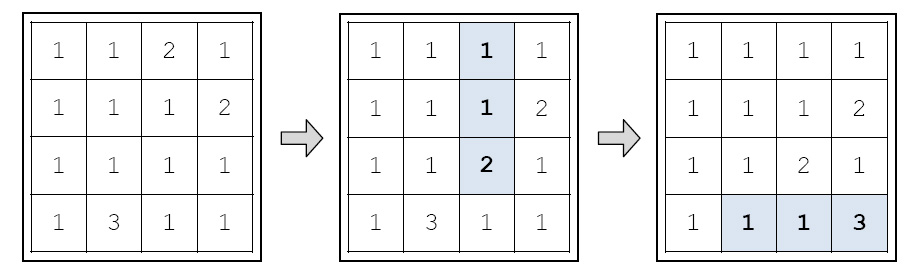
\includegraphics[width=0.7\textwidth]{../latex/img/1081/pic1.jpg}
\end{figure}

 นอกจากนี้เรายังสามารถเผาท่อนไม้เพื่อให้เชื้อเพลิงแต่ละครั้งจะเผาท่อนไม้ที่อยู่ติดกัน $4$ ท่อนในรูปของ $2\times 2$ หน่วยดังรูป
 
 \begin{figure}[h!]
\centering
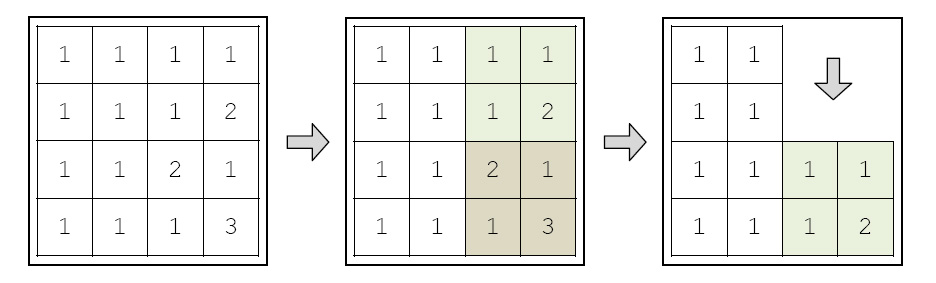
\includegraphics[width=0.7\textwidth]{../latex/img/1081/pic2.jpg}
\end{figure}
 
 จากรูปการเผาท่อนไม้สี่ท่อนครั้งแรก ทำให้ได้พลังงาน $2\times 1\times 1\times 3=6$ หน่วย
 
 เมื่อทำการเผาท่อนไม้ $4$ ท่อนดังกล่าวแล้ว ท่อนไม้ที่ถูกเผาทั้งหมดจะหายไปกลายเป็นเพียงผงเถ้าถ่าน พลังงานที่เกิดจากการเผาท่อนไม้ดังกล่าวเท่ากับผลคูณของมวลของท่อนไม้ทั้งสี่  หลังจากนั้นท่อนไม้ที่เหลือที่อยู่ข้างบนจะตกลงมาอยู่บนท่อนไม้ข้างล่างแทน  ในการเผาท่อนไม้เพื่อให้ได้พลังงานนี้ คุณสามารถเลือกที่สลับท่อนไม้สลับกับการเผาท่อนไม้ได้
 
 คุณต้องการที่จะทราบว่า จะสามารถเผาท่อนไม้ให้ได้พลังงานรวมมากที่สุดโดยใช้การเผาท่อนไม้และการสลับท่อนไม้ในรูปแบบที่กำหนดให้ได้มากที่สุดเท่าไหร่ เพราะถ้าหากพลังงานน้อยเกินไปจะทำให้เตาผิงดับกลางงานเลี้ยง งานเลี้ยงนี้คงจบไม่สวยแน่

\newpage
\bigskip
\underline{\textbf{โจทย์}}   เขียนโปรแกรมที่รับข้อมูลของท่อนไม้แต่ละท่อนในเครื่องเผาผลาญไม้ แล้วหาว่าจะสามารถเผาท่อนไม้ให้ได้พลังงานรวมมากที่สุดเท่าใด

\InputFile

\textbf{บรรทัดแรก} รับจำนวนเต็ม $N$ $(2 \leq N \leq 500)$ บอกขนาดความกว้างและความสูงของถังตามลำดับ

\textbf{บรรทัดที่ $2$ ถึง $N+1$} มีจำนวนเต็มบรรทัดละ $N$ จำนวน ระบุมวลของท่อนไม้แต่ละท่อนในเครื่องเผาพลาญไม้ โดยที่จำนวนเต็มลำดับที่ $j$ ของข้อมูลนำเข้าบรรทัดที่ $i+1$ หรือ $a_{ij}$ ระบุมวลของท่อนไม้ที่อยู่ในแถวที่ $i$ (นับจากบน) คอลัมน์ที่ $j$ โดยมวลของท่อนไม้แต่ละท่อนเป็นจำนวนเต็มบวกที่มีหลักเดียว $(1 \leq a_{ij} \leq 9)$


\OutputFile

\textbf{มีบรรทัดเดียว} มีจำนวนเต็มหนึ่งจำนวนบอกพลังงานที่มากที่สุดที่สามารถทำได้จากการเผาท่อนไม้ด้วยเงื่อนไขที่กำหนดไว้

\Examples

\begin{example}
\exmp{4
1 1 2 1
1 1 1 1
1 1 1 1
1 3 1 1}{9}%
\end{example}


\Source

สุธี เรืองวิเศษ

\underline{\href{http://www.thailandoi.org/toi.c/02-2009}{TOI.CPP:02-2009}}

\end{problem}

\end{document}